\documentclass{article}
\usepackage[utf8]{inputenc}
\usepackage{minted}
\usepackage{mathtools}
\usepackage{amssymb} 
\usepackage{tabularx}
\usepackage{tabularray}
\usepackage{xcolor}
\usepackage[square,sort,comma,numbers]{natbib}
\renewcommand{\bibsection}{\section{Referências}}
\usepackage[portuguese]{babel}
\usepackage{tikz}
\usetikzlibrary{automata,shapes,arrows,positioning,calc}


\title{Projeto Pesquisa Tratamento Incertezas}
\author{Ewerton Luiz Costadelle \\ Rafael Nink de Carvalho}
\date{26 de agosto de 2022}

\begin{document}

\maketitle

\section{Introduction}


\section{Base de dados}\label{base_de_dados}

Para essa análise foi utilizada uma base de dados com 18.178 observações, do resultado de componentes curriculares ofertadas entre os anos de 2013 e 2020. Essa base foi extraída a partir de boletins de notas de 506 estudantes de um curso técnico de nível médio. Os alunos frequentam cerca de 16 disciplinas por ano e cada observação refere-se ao resultado individual do aluno em uma disciplina. O curso em questão possuiu dois planos pedagógicos, 4 (quatro) anos para ingressantes até 2013 e em 2014 iniciou-se o curso de 3 (três) anos. De modo que os atributos foram detalhados na tabela abaixo: \\

\begin{longtblr}[
    caption = {Boletins dos estudantes},
    label = {boletins},
  ]{
    colspec = {|l|l|X|},
    rowhead = 1,
    hlines,
    row{even} = {lightgray},
    row{1} = {gray},
  } 
  \textbf{Campo} & \textbf{Tipo} & \textbf{Descrição} \\
  ano & Numérico & Ano da observação [2013-2020]\\ 
  periodo & Numérico & Periodo letivo no ano observado [1-4]\\ 
  estudante & Nominal & Identificação anonimizada do estudante\\ 
  disciplina & Nominal & Componente curricular da observação\\ 
  ch & Numérico & Número de aulas programadas por ano na disciplina [0-120]\\ 
  tipo & Nominal & As matriculas podem ser regulares ou especiais.\\ 
  anp & Numérico & Número de aulas não presenciais no ano [0-120]\\ 
  aulas & Numérico & Numero de aulas presenciais registradas [0-120]\\ 
  faltas & Numérico & Quantidade de faltas no final do ano letivo [0-120]\\ 
  justificadas & Numérico & Quantidade de faltas com justificativa legal no final do ano letivo [0-120]\\ 
  percentual & Numérico & Percentual de frequencia do estudante [0-100\%]\\ 
  nb1 & Numérico & Nota do 1º bimestre na componente curricular [0-100]\\ 
  nb2 & Numérico & Nota do 2º bimestre na componente curricular [0-100]\\ 
  ms1 & Numérico & Média aritmética das notas de 1º e 2º bimestres. Estudantes com média abaixo de 60 pontos são convocados para estudo de recuperação, do 1º semestre [0-100]\\ 
  nr1 & Numérico & Nota obtida no estudo de recuperação do 1º semestre [0-100]\\ 
  mr1 & Numérico & Média calculada após o estudo de recuperação. Até 2015 era a média entre ms1 e nr1. Em 2016, passou a ser substitutiva, quando nr1 é maior que ms1 [0-100]\\ 
  nb3 & Numérico & Nota do 3º bimestre na componente curricular [0-100]\\ 
  nb4 & Numérico & Nota do 4º bimestre na componente curricular [0-100]\\ 
  ms2 & Numérico & Média aritmética das notas de 3º e 4º bimestres. Estudantes com média abaixo de 60 pontos são convocados para estudo de recuperação, do 2º semestre [0-100]\\ 
  nr2 & Numérico & Nota obtida no estudo de recuperação do 2º semestre [0-100]\\ 
  mr2 & Numérico & Média calculada após o estudo de recuperação. Até 2015 era a média entre ms2 e nr2. Em 2016, passou a ser substitutiva, quando nr2 é maior que ms2 [0-100]\\ 
  ma & Numérico & Média aritmética entre mr1 e mr2. Estudantes com média abaixo de 60 pontos são ocnvocados para exame final.\\ 
  nef & Numérico & Nota obtida no exame final [0-100]\\ 
  mf & Numérico & É média ponderado de 60\% da nota da ma com 40\% da nef [0-100]\\
  resultado & Categórico & Estudantes com nota mf maior ou igual a 50 pontos são considerados aprovados, caso contrários, reprovados [ap, ac, rt, rf]\\
  resultado ano & Categórico & Até 2015, estudantes eram considerado aprovados caso ficassem retidos em 3 ou menos e podiam cursar cursá-las em regime de dependência. Em 2016, estudantes podem ser aprovados em conselhos de classe [Aprovado, Reprovado]\\ 
  situação atual & Categórico & Situação atual (2022) do estudante no sistema acadêmico [Matriculado, Concluído, Transferência externa, Evadido, Jubilado]
\end{longtblr}

\begin{tabular}{l r r}
    Aprovado & 911\\
    Reprovado & 233\\
    \textbf{Total} & \textbf{1144}
\end{tabular}

\subsection{Agregação dos dados}\label{agregacao_dos_dados}

As notas das disciplinas foram agregadas por ano, a fim de reduzir o ruido. De modo que, a média de todas as notas do 1º bimestre formou o índice de rendimento acadêmico (\texttt{ira\_nb1}). Para as etapas posteriores a formação do índice considera a situação do estudante naquele momento. Para o \texttt{ira\_mr1}, é considerado a média aritmética entre as notas do 1º e 2º bimestres, ou a nota da recuperação, caso seja superior. Para o \texttt{ira\_nb3} foi feito uma média ponderada considerando dois terços da média após recuperação e um terço da nota do 3º bimestre. Nesse sentido, a cada passo o rendimento acadêmico pode ser mensurado, considerando as etapas anteriores.

O algoritmo de A Tabela \ref{agregado} foi com 


\begin{longtblr}[
    caption = {Dados agregados},
    label = {agregado},
  ]{
    colspec = {|l|l|X|},
    rowhead = 1,
    hlines,
    row{even} = {lightgray},
    row{1} = {gray},
  } 
  \textbf{Campo} & \textbf{Tipo} & \textbf{Descrição} \\
    ano & Numérico & Ano da observação [2013--2020]\\ 
    periodo & Numérico & Periodo letivo no ano observado [1--4]\\ 
    estudante & Nominal & Identificação anonimizada do estudante\\ 
    ira\_nb1 & Numérico & Média das notas do 1º bimestre \\
    ira\_mr1 & Numérico & Média das notas após a recuperação semestral\\
    ira\_nb3 & Numérico & Média ponderada de dois terços da média após recuperação e um terço da nota do 3º bimestre\\
    rec\_s1 & Numérico & Quantidade de disciplinas em que o estudante foi convocado para estudos de recuperação no 1º semestre\\
    rec\_s2 & Numérico & Quantidade de disciplinas em que o estudante foi convocado para estudos de recuperação no 2º semestre\\
    qtd\_disciplinas & Numérico & Quantidade de disciplinas que o estudante cursou no ano\\
    ap & Numérico & Quantidade de disciplinas aprovadas\\
    ac & Numérico & Quantidade de disciplinas aprovadas com o recurso do conselho de classe\\
    rt & Numérico & Quantidade de disciplinas em que o estudante ficou retido por nota\\
    rf & Numérico & Quantidade de disciplinas em que o estudante ficou retido por falta\\
    resultado\_final & Categórico & Até 2015, estudantes eram considerado aprovados caso ficassem retidos em 3 ou menos e podiam cursar cursá-las em regime de dependência. Em 2016, estudantes podem ser aprovados em conselhos de classe [Aprovado, Reprovado]\\ 
    situacao\_atual & Categórico & Situação atual (2022) do estudante no sistema acadêmico [Matriculado, Concluído, Transferência externa, Evadido, Jubilado] \\
    grupo & Categórico & Informação qualitativa do estudante no ano. A: concluiu o ano letivo com êxito, sem recuperações; B: concluiu o ano letivo com êxito, com pelo menos uma recuperação, sem aprovação por conselho de classe ou dependência; C: concluiu o ano letivo com êxito, com pelo menos uma aprovação por conselho de classe ou dependência; D: retido por nota ou por falta em até 3 disciplinas; e E: retido por falta em 4 ou mais disciplinas.\\
\end{longtblr}

  
\subsection{Cadeia de Markov}\label{cadeia_de_markov}

\begin{center}
\begin{tikzpicture}[->, >=stealth', auto, semithick, node distance=2cm]

\node[state] (Input)                             {Início};
\node[state] (C)            [below of = Input]   {AC};
\node[state] (B)            [left of = C]        {AP};
\node[state] (A)            [left of = B]        {A+};
\node[state] (D)            [right of = C]       {RT};
\node[state] (E)            [right of = D]       {RF};

\node[state] (AA)            [below of = A]        {A+};
\node[state] (BB)            [below of = B]        {AP};
\node[state] (CC)            [below of = C]        {AC};
\node[state] (DD)            [below of = D]        {RT};
\node[state] (EE)            [below of = E]        {RF};

\node[state] (AAA)            [below of = AA]        {A+};
\node[state] (BBB)            [below of = BB]        {AP};
\node[state] (CCC)            [below of = CC]        {AC};
\node[state] (DDD)            [below of = DD]        {RT};
\node[state] (EEE)            [below of = EE]        {RF};

\node[state] (Concluido)    [below of = BBB]       {Concluído};
\node[state] (Evadido)      [right of = EE]       {Evadido};

\node   [left of = A]        {1º};
\node   [left of = AA]       {2º};
\node   [left of = AAA]      {3º};


\path(Input) edge[bend right]   node{6.1\%}   (A);
\path(Input) edge[]   node{45.3\%}   (B);
\path(Input) edge[]   node{16.3\%}   (C);
\path(Input) edge[]    node{26.5\%}   (D);
\path(Input) edge[bend left]    node{5.7\%}   (E);

\path(E)     edge[bend left]   node{93.8\%}   (Evadido);
\path(E)     edge[bend left]   node{6.2\%}   (D);


\path(D)     edge[bend left]   node{2.4\%}   (E);
\path(D)     edge[loop below]  node{21.4\%}   (D);
\path(D)     edge[bend left]   node{14.3\%}   (C);
\path(D)     edge[bend left]   node{25.0\%}   (B);
\path(D)     edge[bend left]   node{36.9\%}   (Evadido);


\path(C)     edge[bend left]   node{17.3\%}   (DD);
\path(C)     edge[loop  below]  node{21.2\%}   (CC);
\path(C)     edge[bend right]  node{23.1\%}   (BB);
\path(C)     edge[bend left]   node{38.5\%}   (Evadido);



\path(AAA)     edge[bend right]  node{100.0\%}   (Concluido);
\path(BBB)     edge  node{100.0\%}   (Concluido);
\path(CCC)     edge[bend left]  node{100.0\%}   (Concluido);

[0.057, 0.265, 0.163, 0.453, 0.061]

 [[[0.0, 0.062, 0.0, 0.0, 0.0, 0.0, 0.938],
   [0.024, 0.214, 0.143, 0.25, 0.0, 0.0, 0.369],
   [0.0, 0.173, 0.212, 0.231, 0.0, 0.0, 0.385],
   [0.008, 0.098, 0.152, 0.629, 0.03, 0.0, 0.083],
   [0.0, 0.067, 0.0, 0.4, 0.533, 0.0, 0.0]],
   
  [[0.333, 0.0, 0.0, 0.0, 0.0, 0.0, 0.667],
   [0.042, 0.042, 0.125, 0.292, 0.0, 0.0, 0.5],
   [0.059, 0.206, 0.206, 0.353, 0.029, 0.0, 0.147],
   [0.0, 0.019, 0.111, 0.722, 0.074, 0.0, 0.074],
   [0.0, 0.0, 0.0, 0.5, 0.5, 0.0, 0.0]],
   
  [[0.0, 0.5, 0.0, 0.0, 0.0, 0.0, 0.5],
   [0.0, 0.0, 0.0, 0.1, 0.0, 0.0, 0.9],
   [0.0, 0.0, 0.0, 0.0, 0.0, 1.0, 0.0],
   [0.0, 0.0, 0.0, 0.0, 0.0, 1.0, 0.0],
   [0.0, 0.0, 0.0, 0.0, 0.0, 1.0, 0.0]]])

\end{tikzpicture}
\end{center}



\[
\begin{bmatrix}
\pi_{0} \\
\pi_{1} \\
\pi_{2} \\
\pi_{3} \\
\pi_{4} \\
\pi_{5} \\
\pi_{6}
\end{bmatrix}^T \times
\begin{bmatrix}
    1   & 0 & 0 & 0 & 0 & 0 & 0 \\
    1-p & 0 & p & 0 & 0 & 0 & 0 \\
    0 & 1-p & 0 & p & 0 & 0 & 0 \\
    0 & 0 & 1-p & 0 & p & 0 & 0 \\
    0 & 0 & 0 & 1-p & 0 & p & 0 \\
    0 & 0 & 0 & 0 & 1-p & 0 & p \\
    0 & 0 & 0 & 0 & 0 & 0 &   1 \\
\end{bmatrix} =
\begin{bmatrix}
\pi_{0} \\
\pi_{1} \\
\pi_{2} \\
\pi_{3} \\
\pi_{4} \\
\pi_{5} \\
\pi_{6}
\end{bmatrix}^T
\]

\section{Um segundo método para a predição} \label{sec:firstpage}

Inicialmente, pensou-se em utilizar árvores de decisão, porque são estruturas muito simples e com alto grau de interpretabilidade. Esse método, utilizado tanto para classificação quanto para regressão, foi proposto há quase 60 anos por \cite{Morgan_1963} e desde então teve muitas variações.

Basicamente, uma árvore é uma estrutura hierárquica que particiona dados de modo a torná-los mais homogêneos possível. Ela subdivide um conjunto amostral com base nos seus atributos. É mais intuitiva a seleção de atributos categóricos, porém, atributos numéricos carecem de uma definição do melhor ponto para fazer o corte. No exemplo da Figura \ref{Fig1} o nó raiz particiona o conjunto de flores pela largura de suas pétalas. Ainda no exemplo, serão direcionadas ao nó da esquerda aquelas que tiverem largura menor que 2.45. Consequentemente, larguras maiores ou iguais a 2.45 serão direcionadas ao nó da direita, de modo que novos particionamentos podem ser feitos, até que nós folhas sejam tão homogêneos quanto o desejado. E é majoritariamente, no modo como o algoritmo faz esse particionamento é que define qual é o seu modelo.

\begin{figure}[ht]
\centering
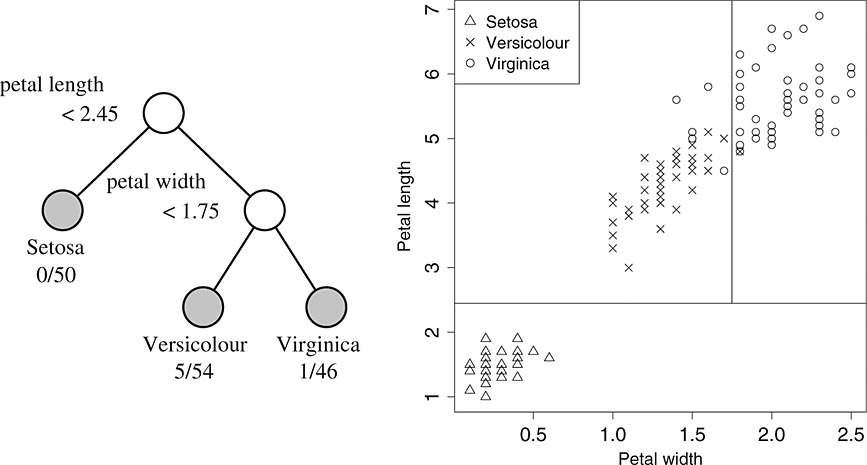
\includegraphics[width=.5\textwidth]{fig1.png}
\caption{Exemplo de uma árvore de decisão. Fonte \cite{Loh_2014}}
\label{Fig1}
\end{figure}

O modelo AID (\emph{Automatic Interaction Detection}) proposto por \cite{Morgan_1963}, varre o vetor do atributo sempre separando o conjunto em dois. A cada particionamento é calculado o erro pelo método dos mínimos quadrados. O ponto de partição que obtiver menor erro é o selecionado. A seleção da raiz de uma subárvore também é baseada no erro quadrático médio, após obter o ponto de corte e o erro de todos os atributos, seleciona-se a raiz. O processo é iterado até que se atinja condições de seleção definidas previamente.

Outros modelos acrescentaram padrões utilizados até os dias de hoje, o THAID (\emph{THeta Automatic Interaction Detection}) \cite{Messenger1972} introduziu os conceitos de entropia e índice de Gini na seleção do nó raiz. E o CART (\emph{Classification And Regression Trees}), proposto por \cite{Breiman1984}, utilizou divisões em combinações lineares de variáveis, por busca estocástica e resolveu problemas de valores de dados ausentes em um nó.

O algoritmo  \textit{Iterative Dichotomiser} 3 (ID3) introduzido  por  \cite{quinlan1986} é elaborado a partir de uma sistemas de inferência, gerando uma árvore da raiz às folhas usando o ganho de informação para definir a melhor raiz, de forma recursiva encontra-se o melhor filho, ou seja, o atributo que melhor divide o conjunto de dados, seguindo até as folhas. Possui limitação quanto aos tipos de dados, sendo necessário que este sejam categóricos não ordinais, desta forma o C4.5 apresenta-se como uma evolução trabalhando com dados contínuos, além de tratar dados desconhecidos, ou seja, não presente nos dados de testes, ainda apresenta um método de pós-poda para avaliar desempenho.

\subsection{Das métricas}

Diversas métricas são comumente utilizadas na construção das árvores de decisão, como: grau de entropia, ganho de informação

O grau de entropia, dada uma amostra(S) com resultados positivos (+) e negativos (–) de algum conceito alvo, para uma classificação booleana definido pela expressão é
\begin{equation}
    Entropia(S) \equiv -p_+ \log_2 p_+ - p_- \log_2 p_-
\end{equation}
tendo como resultados no intervalo $[0,1]$, quanto mais próximos de 1, menor a dúvida na classificação.

De forma genérica, se atributo alvo aceitar $c$ diferentes valores, a entropia de $S$ relativa a esta classificação c–classes é definida como:
\begin{equation}
    Entropia(S) \equiv \sum_{i=1}^{c} -p_i \log_2 p_i
\end{equation}
sendo $p_i$ a proporção de $S$ pertencendo a classe $i$.

Neste contexto a entropia refere-se a aleatoriedade de uma variável prever a classe,  enquanto a métrica ganho de informação representa a redução da entropia causada pela divisão dos exemplos de acordo com os valores do atributo, sendo expressa:
\begin{equation}
    Gain(S,A) \equiv Entropia(S) - \sum_{v \in valores(A)} \frac{|S_v|}{|S|} Entropia(S_v)
\end{equation}
redução esperada na entropia causada gerada pela divisão dos exemplos de acordo com este atributo A.


\subsection{Submétodos combinados para formar uma floresta}

O \textit{Random Forest}, é um algoritmo híbrido, que além de árvores de decisão, utiliza de métodos de agregação e a subdivisão do espaço amostral. Utiliza o \textit{Bagging}, que é um método de estimação de parâmetros com alto poder de extrair informação dos dados. Nesse contexto, seria um erro traduzir \textit{bagging} com qualquer variação do verbo empacotar, principalmente porque pouco teria a ver com a ideia que o motiva. De fato, o autor \cite{Breiman_1996} o descreveu como o acrônomio de \emph{\textbf{b}ootstrap} \emph{\textbf{agg}regat\textbf{ing}}, ou seja, é um agregador de preditores baseados na técnica \textit{bootstrap} de reamostragem. 

Por sua vez, o \textit{bootstrap} é uma técnica de reamostragem proposta por \cite{Efron_1993} que consiste em remover e repor aleatoriamente uma porcentagem de amostras de um conjunto de dados para estimar alguns parâmetros. Com base no novo conjunto de dados, problemas como a falta de normalidade são contornados, permitindo a inferência estatística e determinação de parâmetros, como intervalos de confiança, de modo analítico. É um método estatístico que ficou popular com o aumento do poder computacional, principalmente a partir da década de 1990.

No código, abaixo, um conjunto de dados com tamanho amostral $n=6$ foi reamostrado $N_{boot}=400$ vezes. O sorteio foi feito utilizando o gerador de números pseudo-aleatórios da biblioteca \textit{NumPy}\cite{Harris_2020}. De modo que, $x$ armazena os índices (randomizados) que compuseram o novo conjunto de dados. Nesse sentido, a complexidade assintótica do método depende de $O(N_{boot}) \times O(n)$, ou simplesmente, $O(n)$.

\begin{listing}[!ht]
\begin{minted}[frame=lines,fontsize=\footnotesize]{python}
import numpy as np
porosity = [30.3, 21.0, 19.2, 29.1, 21.9, 23.1]
Nboot = 400
def bootstrap(x, Nboot, statfun):
    x = np.array(x)
    resampled_stat = []
    for b in range(Nboot):
        index = np.random.randint(0,len(x),len(x))
        sample = x[index]
        bstatistic = statfun(sample)
        resampled_stat.append(bstatistic)
    return np.array(resampled_stat)
porosity_bootstrap = bootstrap(porosity, Nboot, np.mean)
\end{minted}
\caption{Exemplo de \emph{bootstrapping} em Python}
\end{listing}


No caminho de explicar a origem do nome, os autores do método de \textit{bootstrap} \cite{Efron_1993} o referenciaram a um conto alemão do século XVIII denominado As Aventuras do Barão de Münchhausen (em tradução livre), de Rudolph Erich Raspe. Em um trecho do livro, o barão escapa de um pântano puxando (a si próprio) pela cinta das próprias botas. É uma alegoria que tenta retratar algo, ou alguém, que consegue evoluir partindo do nada e pelos próprios meios.

Uma outra alegoria que circunda o tema está na na conclusão do artigo denominado \emph{Bagging Predictors}. O autor \cite{Breiman_1996} utiliza o contrassenso de um provérbio dizendo que utilizar o método de \emph{Bagging} em preditores, é uma maneira de fazer "uma bolsa de seda a partir da orelha de uma porca" e completa, "especialmente se a orelha da porca estiver trêmula". 

Na prática, o que o método de \emph{Bagging} faz é produzir varias versões do conjunto de amostras para depois criar conjuntos de treino $\mathcal{L}$ e teste $\mathcal{T}$. Para se ter noção, no artigo que apresentou o método, o autor transformou um conjunto de 200 amostras em 2000, de modo que, 200 foram utilizadas como treinamento de uma árvore de decisão e 1800 como teste.

Nesse sentido, um conjunto de árvores com \textit{bagging} (\textit{Bagging Trees}) é um método em que na construção de cada árvore é feita uma seleção aleatória a partir dos exemplos do conjunto de treinamento. 

Ampliando, surge a possibilidade de escolha aleatória de $n$ diferentes subconjuntos de preditores, a partir do espaço de preditores original, para treinar $n$ classificadores, com isso, cada elemento do conjunto será treinado com apenas uma porção das preditores, permitindo classificar uma amostra com preditores ausentes ao selecionar os elementos do conjunto treinados somente com os preditores disponíveis no dado a ser classificado, esse método é chamado de subespaço aleatório \cite{polikar2010}. 

\subsection{Floresta de árvores aleatórias}

Nesse sentido, em uma floresta de árvores aleatórias (\textit{Random Forest}) há uma combinação de preditores de árvores de modo que cada árvore depende dos valores de um vetor aleatório amostrado independentemente e com a mesma distribuição para todas as árvores da floresta \cite{Breiman_2001}.

O Scikit-learn \cite{scikit-learn} é uma das mais populares bibliotecas para fazer aprendizado de máquina em Python \cite{Grus_2019}. Seus pacotes contêm diversos módulos, dos quais pode-se citar o \texttt{sklearn.tree}, onde estão os módulos necessários para árvores de decisão e, para florestas de árvores, o \texttt{sklearn.ensemble}.

A complexidade assintótica do \emph{Random Forest}, sem limitações é $O(M\cdot N \cdot\log{N})$, onde $M$ é o número de árvores e $N$ é o número de amostras. É possível reduzir a complexidade alterando parâmetros que limitem o número mínimo de amostras para que o nó seja particionado (\texttt{min\_samples\_split}), o número máximo de nós folhas (\texttt{max\_leaf\_nodes}), a altura das árvores (\texttt{max\_depth}) e o número mínimo de amostras nas folhas (\texttt{min\_samples\_leaf}).

A utilização é facilitada e basta inserir alguns parâmetros e a biblioteca encarrega-se do restante. Na sequência tem-se o código-fonte que carrega um conjunto de dados, seleciona-se os preditores e alvo, separa a base de teste, executa o algoritmo do Random Florest e por fim realiza a impressão da análise.


\begin{listing}[H]
\begin{minted}[frame=lines,fontsize=\footnotesize,breaklines,autogobble]{python}
import pandas as pd
from sklearn.model_selection import train_test_split
from sklearn.metrics import accuracy_score
from sklearn.metrics import recall_score
from sklearn.metrics import confusion_matrix
from sklearn.ensemble import RandomForestClassifier

github = (
    'https://raw.githubusercontent.com/ecostadelle/'+
    'ProjetoPesquisaTratamentoIncertezas/main/db/transforma.csv')
df = pd.read_csv(github, sep = ';',decimal=",")
X = df[['ira_nb1', 'ira_mr1', 'ira_nb3', 'rec_s1']]
y = y=df[['resultado_final']]

X_train, X_test, y_train, y_test = train_test_split(X, 
                                                    y, 
                                                    test_size=0.25, 
                                                    random_state=123)
rfc = RandomForestClassifier(bootstrap=True,
                             n_estimators=10,
                             max_depth=None,
                             min_samples_split=2,
                             random_state=0)
rfc.fit(X_train, y_train.values.ravel())
y_pred=rfc.predict(X_test)
\end{minted}
\caption{Exemplo de \emph{Random Forest} utilizando o Scikit-learn}
\end{listing}

No código-fonte anterior o parâmetro \textit{n\_estimators} define o número de árvores que serão geradas e a impressão destas pode ser feito pelo código-fonte que segue:

\begin{listing}[H]
\begin{minted}[frame=lines,fontsize=\footnotesize,breaklines]{python}
from dtreeviz.trees import dtreeviz
from sklearn import tree
from matplotlib import pyplot as plt
plt.rcParams.update({'figure.figsize': (12.0, 8.0)})
plt.rcParams.update({'font.size': 14})
plt.figure(figsize=(20,20))
_ = tree.plot_tree(rfc.estimators_[0], 
                    feature_names=X.columns,
                    filled=True)
\end{minted}
\caption{Exemplo de Impressão de \emph{Random Forest} utilizando o Scikit-learn}
\end{listing}

Ao executar o código-fonte supracitado gera-se uma árvore escolhida no parâmetro \texttt{n\_estimators}, sendo um exemplo, a árvore a seguir. 

\begin{figure}[H]
\centering
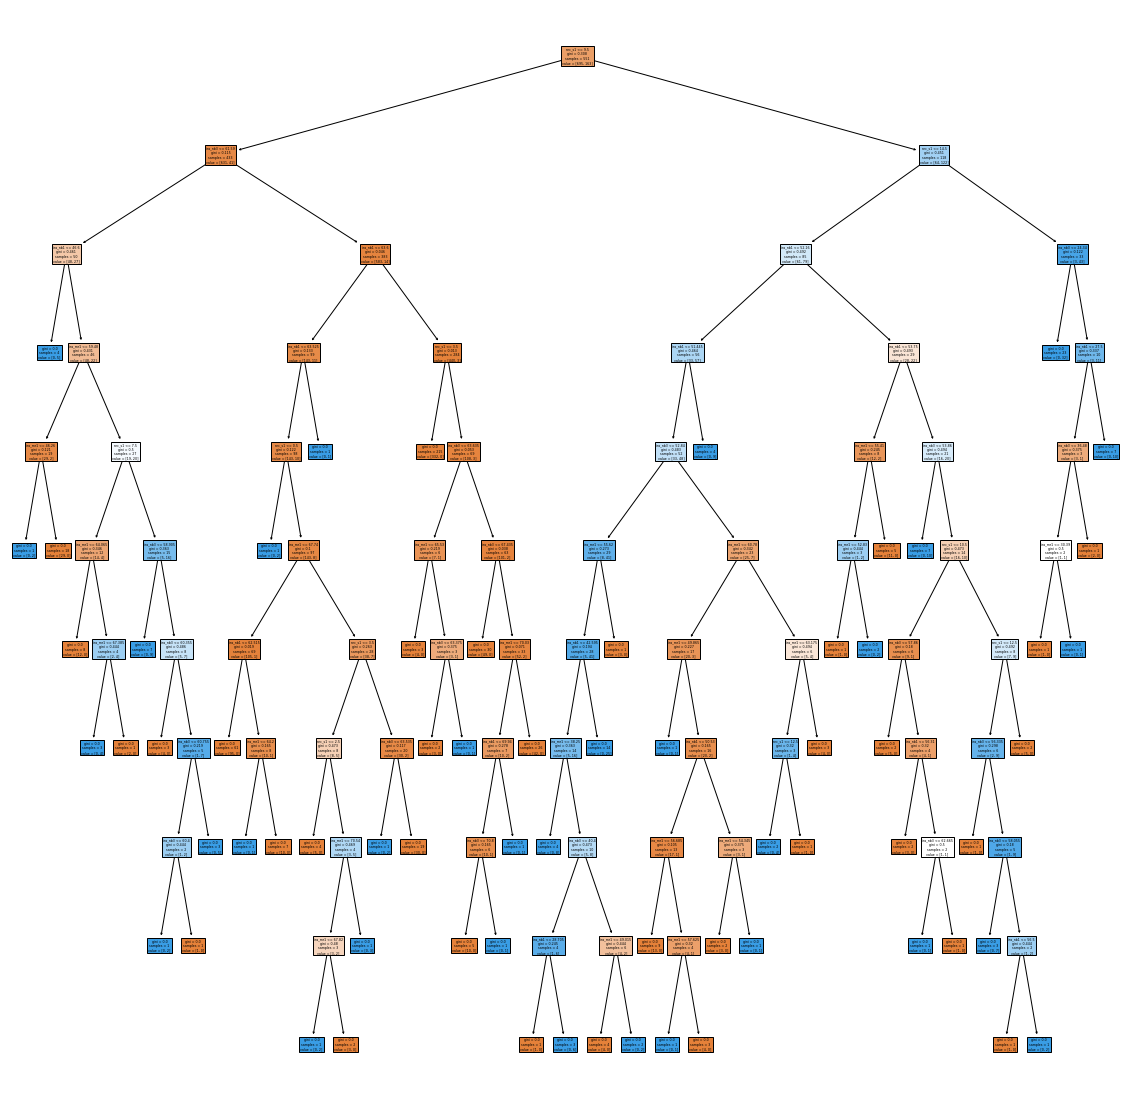
\includegraphics[width=1\textwidth]{tree_0.png}
\caption{Arvore 0 [0,9] do modelo treinado}
\label{Tree}
\end{figure}

\section{Resultados e discussões}

\section{Conclusões}
		
\bibliographystyle{acm}
\bibliography{main}
 
\end{document}
